\documentclass[mathserif]{beamer}
\usepackage[english]{babel}
\usepackage{amsmath,amsthm, amssymb}

\usetheme{DCNposter} 
\usepackage[orientation=portrait,size=a0,scale=1.0]{beamerposter}  % you can change the scale to 1.0 if you have more text. 

\title{Stochastic simulation and optimization \\ for dynamical systems} % Title will always appear in italics
\author{Dani\"el Veldman, Enrique Zuazua} 
\institute{Chair in Dynamics, Control, and Numerics -- 
AvH-Professorship, Dept.\ of Data Science, Friedrich-Alexander-University Erlangen-N\"urnberg}
\date{\today}
% author, institute, and date are not yet used in the template. This should still be improved. 
% It is better to define authors and institute anyway, because it will appear in the properties of the pdf

\begin{document}
\begin{frame}
%
% PUT YOUR CONTENT HERE:
% you can of course modify the columns and content as you like, this is just an example. 
\vspace{0.4cm}

\begin{columns}[T]
\begin{column}{0.45\textwidth}
    \begin{columns}
    \begin{column}{0.15\textwidth}    
    \bf Dani\"el \\ Veldman
    \end{column}
    \begin{column}{0.82\textwidth}    
    Chair in Dynamics, Control, and Numerics -- AvH Professorship \\
    FAU Erlangen-Nürnberg
    \end{column}
    \end{columns}
\end{column}
    
\begin{column}{0.45\textwidth}
    \begin{columns}
    \begin{column}{0.15\textwidth}    
    \bf Enrique \\ Zuazua
    \end{column}
    \begin{column}{0.82\textwidth}    
    Chair in Dynamics, Control, and Numerics -- AvH Professorship \\
    FAU Erlangen-Nürnberg
    \end{column}
    \end{columns}
\end{column}
\end{columns}

\vspace{1.1cm}

\begin{columns}[T]
    \begin{column}{.45\textwidth}
    
      \begin{block}{Introduction}
      Stochastic optimization techniques such as the Random Batch Method (RBM) are well-established and widely used in modern intelligent systems such as search engines, recommendation software, and speech and image recognition platforms [1].  
         
      The RBM has also been applied to the simulation and optimization of interacting particle systems where it leads to a significant reduction in computational cost [2,3]. Inspired by these results, we consider here a stochastic method to speed up the simulation and optimization of large-scale linear dynamical systems. 
      \end{block}   
   
      \begin{block}{Optimal control}
      In a classical control problem, the aim is to find the optimal control $u^*(t)$ that minimizes
      \begin{equation}
      J = \int_0^T \left( (x(t)-x_d(t))^\top Q (x(t)-x_d(t)) + u(t)^\top R u(t) \right) \ \mathrm{d}t, \label{eq:cost_x}
      \end{equation}
      on a finite time interval $[0,T]$ subject to the dynamics
	  \begin{equation}
	  \dot{x}(t) = Ax(t) + Bu(t), \qquad \qquad x(0) = x_0, \label{eq:dyn_x}
	  \end{equation}
      where $x(t) \in \mathbb{R}^N$ is the state, $u(t) \in \mathbb{R}^q$ is the control,  $x_d(t)$ is a given desired trajectory, and $Q \succeq 0$, $R \succ 0$, $A$, and $B$ are constant matrices. Without loss of generality, we can assume that $q \leq N$. 
      \\
      It is well known that the problem \eqref{eq:cost_x}--\eqref{eq:dyn_x} has a unique solution $u^* \in L^2(0,T; \mathbb{R}^q)$. \\
      However, computing $u^*$ can be challenging because \eqref{eq:dyn_x} and the corresponding adjoint equation need to be solved several times and each time step typically has a computational complexity of $O(N^3)$. 
      
\begin{center}
\textbf{Especially when $N$ is large, finding $u^*(t)$ is computationally demanding. } 
\end{center}      
      \end{block}  
      
      \begin{block}{Stochastic simulation and optimization method}
\begin{description}
\item[Step 1] Decompose the matrix $A$ into  submatrices $A_m$ as
      \begin{equation}
      A = \sum_{m=1}^M A_m. \label{eq:sumA}
      \end{equation}
      The submatrices $A_m$ are chosen such that replacing $A$ by $A_m$ in \eqref{eq:dyn_x} reduces the computational cost per time step. Typically, the submatrices $A_m$ will be more sparse than $A$. 
      \item[Step 2] Let $\{ \mathcal{S}_\ell \}_{1 \leq \ell \leq 2^M}$ denote the collection of $2^M$ subsets of $\{ 1,2, \ldots, M \}$. \\
      Assign to each subset a probability $p_\ell \in [0,1]$  with which the subset $\mathcal{S}_\ell$ will be selected such that
		\begin{itemize}
		\item $\sum_{\ell=1}^{2^M} p_\ell = 1$,
		\item $\pi_m = \sum_{\{ \ell \mid m \in \mathcal{S}_\ell \} } p_\ell > 0$ for each $m \in \{1,2, \ldots , M \}$.
\end{itemize}		      
      Note that $\pi_m$ is the probability that the index $m$ is an element of the selected subset. 
      \item[Step 3] Partition the time interval $I = [0,T]$ into $K$ subintervals $I_k = [t_{k-1}, t_k]$ of length $\leq h$. In each time interval $I_k$, choose a subset $\mathcal{S}_{\ell(k)}$ according to the probabilities $p_\ell$ from Step 2 and define
      \begin{equation}
      A_h(t) = \sum_{m \in \mathcal{S}_{\ell(k)}} \frac{A_m}{\pi_m}, \qquad \qquad t \in I_k.
      \end{equation}
      This definition ensures that $\mathbb{E}[A_h(t)] = A$ for all $t \in [0,T]$. 
      \item[Step 4] Find the optimal control $u_h^*(t)$ that minimizes 
      \begin{equation}
      J_h = \int_0^T \left( (x_h(t)-x_d(t))^\top Q (x_h(t)-x_d(t)) + u_h(t)^\top R u_h(t) \right) \ \mathrm{d}t,
      \label{eq:cost_xh}
      \end{equation}
      subject to the dynamics
	  \begin{equation}
	  \dot{x}_h(t) = A_h(t)x_h(t) + Bu_h(t),  \qquad \qquad x(0) = x_0. \label{eq:dyn_xh}
	  \end{equation}  	  
\end{description}     

When the $N \times N$-matrix $A$ is decomposed into $M$ blocks of size $N/\sqrt{M} \times N/\sqrt{M}$, the computational complexity for each time step of \eqref{eq:dyn_xh} and the corresponding adjoint equation is reduced to $O(N^3/M^{3/2})$. 
\begin{center}
\textbf{Typically, $u^*_h(t)$ can be computed faster than $u^*(t)$. }
\end{center}
      \end{block}    
      
      \begin{block}{Convergence results}
      Fix any control $u \in L^2(0,T; \mathbb{R}^q)$ in \eqref{eq:dyn_x}. When the control $u_h(t)$ in \eqref{eq:dyn_xh} is equal to the control $u(t)$ in \eqref{eq:dyn_x}, we can prove similarly as in [3] that 
      \begin{equation}
      \lim_{h \rightarrow 0}\mathbb{E}\left[ |x_h(t) - x(t) |^2\right] = 0, \label{eq:conv_x}
      \end{equation}
      for all $t \in [0,T]$. 
      Using this result and the strong convexity of the cost functional $J_h$, we proved that
      \begin{equation}
      \lim_{h \rightarrow 0} \mathbb{E}\left[ \| u^*_h - u^* \|_{L^2(0,T)}^2 \right] = 0. \label{eq:conv_control}
      \end{equation}

      \begin{center}      
      \vspace{0.5cm}
     \textbf{These results imply that for any $\varepsilon > 0$ and $\delta > 0$, there exists an $h>0$ such that $\mathbb{P}[ \max\limits_{t \in [0,T]} | x_h(t) - x(t) |^2 > \delta] < \varepsilon$ and $\mathbb{P}[\|u^*_h - u^* \|_{L^2(0,T)}^2 > \delta] < \varepsilon$. }
      \end{center}
      
      \end{block}      
    \end{column}
    
    \begin{column}{.45\textwidth}
    \vspace{-0.15cm}
    \begin{block}{Numerical example}
    
    \vspace{0.5cm}
    \begin{columns}
    \begin{column}{0.59\textwidth}
    The temperature in the space $\boldsymbol \xi = (\xi_1, \xi_2, \xi_3) \in [-L,L]^3$ is modeled by the heat equation $y_t = \Delta y$. Our aim is to keep the temperature on $\textcolor{dcnorange}{S_{\mathrm{top}}} = \{ \xi_3 = L \}$ (the \textcolor{dcnorange}{orange} surface in the figure) close to zero by applying a uniform heat load $-\partial y(t,\boldsymbol \xi)/\partial \xi_1 = u(t)$ on $\textcolor{dcngreen}{S_1} = \{ \xi_1 = -L \}$ (the \textcolor{dcngreen}{green} surface in the figure). Zero Neumann boundary conditions are applied except on $\textcolor{dcngreen}{S_1}$. For simplicity, the control $u(t)$ is taken independent of space. The initial condition is $y(0,\boldsymbol \xi) = \exp(-| \boldsymbol \xi |^2 / (8L^2))$ and the cost functional is taken as
    \begin{equation}
    \mathcal{J} = \int_0^T \iint_{\textcolor{dcnorange}{S_{\mathrm{top}}}} y(t,\boldsymbol \xi)^2 \ \mathrm{d}\xi_1  \ \mathrm{d}\xi_2 \ \mathrm{d}t + 10^{-4}\int_0^T u(t)^2 \ \mathrm{d}t.
    \end{equation}
    \end{column}
    
	\begin{column}{0.37\textwidth}
	\begin{center}
	Considered spatial domain
	\vspace{1cm}
	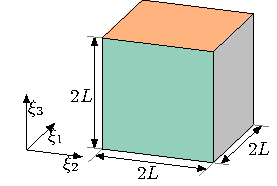
\includegraphics[width=\columnwidth]{Figures/Example.pdf}
	\end{center}
	\end{column}
	
	\end{columns}
	
	\vspace{0.1cm}
The time horizon is $T = 2$ and $L = 1.5$. A finite difference discretization on a uniform rectangular grid with $N = 31^3 = 29,791$ nodes results in a system of the form \eqref{eq:cost_x}--\eqref{eq:dyn_x}. The time grid is uniform with stepsize $h$. 
	Observe that the matrix $A$ can be written as the sum of interaction matrices $A_{ij}$ of the form
      \begin{equation}
      A_{ij}[i,i] = A_{ij}[j,j] = -\tfrac{1}{\Delta \xi^2}, \qquad A_{ij}[i,j] = A_{ij}[j,i] = \tfrac{1}{\Delta \xi^2},
      \end{equation}
      where $i$ and $j$ are adjacent nodes in the spatial grid with spacing $\Delta \xi$. The set of $86,490$ interaction matrices $A_{ij}$ is randomly partitioned into $M$ subsets of approximately equal size. Each submatrix $A_m$ is the sum of the interaction matrices $A_{ij}$ in one subset. Note that this construction assures that \eqref{eq:sumA} holds.  \\
      The probabilities $p_\ell$ are chosen as $p_\ell = 1/M$ when $\mathcal{S}_\ell = \{ m \}$ for some $m \in \{1,2, \ldots , M \}$ and $p_\ell = 0$ otherwise. It follows that $\pi_m = 1/M$. Note that $A_h(t) = A$ when $M = 1$. 
      
      \bigskip
	  We present numerical results for two situations. Situation I illustrates the convergence result \eqref{eq:conv_x} for the solution $x_h(t)$ of the forward dynamics \eqref{eq:dyn_xh} with $u_h(t) = 0$. Situation II illustrates the convergence result \eqref{eq:conv_control} for the control $u_h^*(t)$ that minimizes the cost $J_h$ in \eqref{eq:cost_xh}. In both cases, $x_h(t)$ and $u^*_h(t)$ are computed for $10$ different realizations of the sets $\mathcal{S}_{\ell(k)}$ (but for the same decomposition of $A$ into submatrices $A_m$). The figures below show the mean and the (estimated) $2\sigma$-confidence interval of the error and the computational time (based on these $10$ realizations). Observe that the solutions $x_h(t)$ and $u_h^*(t)$ for $M = 1$ are equal to $x(t)$ and $u^*(t)$. 

\vspace{0.5cm}
\begin{center}      
{Situation I: Relative error and computational time for the response $x_h(t)$ with $u_h(t) = 0$}
\begin{flushright}
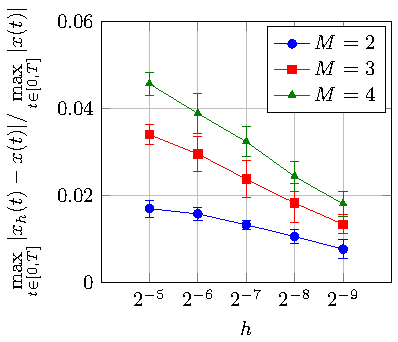
\includegraphics[height=0.435\columnwidth]{Figures/ErrorX.pdf}      
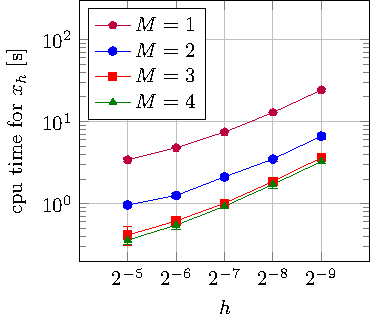
\includegraphics[height=0.41\columnwidth]{Figures/DurationX.pdf}      
\vspace{-0.7cm}
\end{flushright}
\vspace{-0.4cm}
{Situation II: Relative error and computational time for the optimal control $u_h^*(t)$}
\begin{flushright}
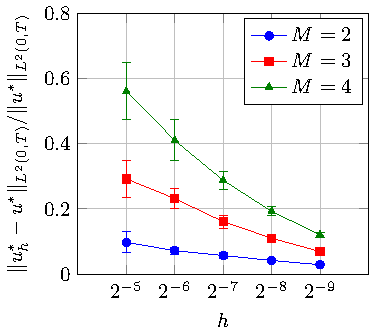
\includegraphics[height=0.425\columnwidth]{Figures/ErrorU.pdf}      
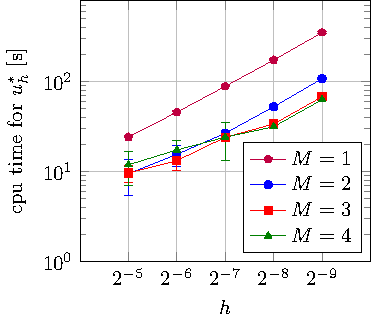
\includegraphics[height=0.41\columnwidth]{Figures/DurationU.pdf}
\end{flushright}
\vspace{-0.7cm}
\end{center}

\vspace{0.2cm}
\begin{center}
\textbf{The figures show that the errors in $x_h(t)$ and $u^*_h(t)$ decrease with $h$. \\
Increasing $M$ increases the error but speeds up the computations. }
\end{center}
      \end{block}
      \end{column}
\end{columns}

\vspace{-0.5cm}
    \begin{columns}[t]
  \begin{column}{0.94\textwidth}
\begin{block}{Conclusions, discussions, and further research}
\vspace{0.5cm}
\begin{columns}
\begin{column}{0.24\textwidth}
The accuracy of the proposed stochastic simulation and optimization method for large-scale linear dynamical systems increases when the time step $h$ is decreased. Our analysis shows that $\mathbb{E}[\max_{t \in [0,T]} | x_h(t) - x(t) |]$ and $\mathbb{E}[\| u_h^* - u^* \|_{L^2(0,T)}]$ converge to zero as $\sqrt{h}$. This rate can also be observed in the numerical example. 
\end{column}

\begin{column}{0.24\textwidth}
In the considered numerical example, the reduction in computational time varies between a factor $2$ and $10$ and generally increases when $h$ decreases. With $M =2$ and $h=2^{-9}$, optimal controls with an expected $4\%$-error are computed $3$ times faster. We expect an even larger reduction in computational time when the state dimension $N$ is increased further. 
\vspace{0.4cm}
\end{column}

\begin{column}{0.24\textwidth}
Note that $x_h$ depends nonlinearly on $A_h$ so that $\mathbb{E}[x_h] \neq x$ and $\mathbb{E}[u^*_h] \neq u^*$ for $h > 0$. Because of this bias, the variation in the $x_h$ and $u^*_h$ obtained for different realizations of the sets $\mathcal{S}_{\ell(k)}$ on the same time grid cannot be used to estimate the expected errors $\mathbb{E}[|x_h(t) - x(t)|^2]$ and $\mathbb{E}[\|u^*_h - u^*\|_{L^2(0,T)}^2]$. 
\vspace{0.9cm} 
\end{column}
    
    \begin{column}{0.24\textwidth}
    Topics for further research:
\begin{itemize}
\item What is the best choice for the probabilities $p_\ell$?
\item What is the best way to decompose $A$ into submatrices $A_m$?
\item Extensions to infinite-dimensional and nonlinear problems. 
\end{itemize}
\vspace{0.9cm} 
\end{column}
\end{columns}
\end{block}
\end{column}
\end{columns}

    \vspace{0cm}
    
\begin{columns}
  \begin{column}{0.94\textwidth}
    \begin{block}{Selected publications}
      \begin{columns}[T]
        \begin{column}{0.24\textwidth}
          [1]\ Bottou, L., Curtis, F. E., Nocedal, J. (2018). {\bf Optimization methods for large-scale machine learning.} Siam Review, 60(2), 223-311.
        \end{column}
        \begin{column}{0.24\textwidth}
          [2]\ Ko, D., Zuazua, E. (2020). {\bf Model predictive control with random batch methods for a guiding problem.} arXiv:2004.14834.
        \end{column}
        \begin{column}{0.24\textwidth}
          [3]\ Jin, S., Li, L., Liu, J. G. (2020). {\bf Random Batch Methods (RBM) for interacting particle systems.} J. Comput. Phys., 400, 108877.
        \end{column}
        \begin{column}{0.24\textwidth}
          [4]\ Veldman, D.W.M., Zuazua, E. {\bf Stochastic time-splitting methods in optimal control.} \\ In preparation. 
        \end{column}
      \end{columns}
    \end{block}
  \end{column}
\end{columns}

\end{frame}
\end{document}
